\chapter{Integreren van Ollama met documentdatabase}

Nu we een geordende documentendatabase hebben, is het tijd om een LLM (Large Language Model) te configureren zodat het kan werken via RAG en zich zal voordoen als een digitale assistent.

Eerst hebben we een retrieval systeem nodig.
Dit is essentieel om queries naar onze database te sturen en chunks op te halen en terug te geven.
Deze documenten worden dan samengevoegd met de query van de gebruiker en gebruikt als parameters voor een Large Language Model. µ

\section{Retrievalsysteem}
\subsection{Werking}
Een retrievalsysteem haalt (om het simpel uit te leggen) data op uit een set data die 'overeenstemt' met de query.
Maar wat is een gelijkenis? Hoe gelijk?
Hoe gaan we documenten vergelijken? Laten we het eens op een rijtje zetten.

\subsection{Retrievalmodellen}
Retrievalmodellen zijn wiskundige technieken die toegepast worden in o.a. zoekmachines en deze zijn gemaakt om relevante documenten op te snorren die relevant zijn met de query van de gebruiker.
We zullen hier drie modellen bespreken die veel gebruikt worden.
In realiteit worden er echter meer libraries gebruikt (gevonden op b.v. het LangChain of Huggingface platform, deze zijn forges die toegang bieden tot allerlei implementaties van LLM tot videogeneratie),
waar de keuze van retrievalmodel voor ons al gemaakt is of tijdens runtime dynamisch gekozen wordt.

\begin{enumerate}
	\item \textbf{Booleaanse retrieval:} dit is een van de meest simpele modellen.
	      Het gebruikt booleaanse (OR, AND, NOT) operatoren om een match te evalueren.
	      Dit kan heel efficiënt en snel zijn, maar het heeft een paar beperkingen.
	      Enerzijds heeft het geen manier om gevonden documenten te ordenen op relevantie
	      en anderzijds kan het heel veel irrelevante informatie teruggeven als een query te breed is gesteld.

	\item \textbf{Vectorruimtemodellen:} Deze zijn wat complexer.
	      Ze gebruiken vectoren, dit zijn documenten en queries die voorgesteld worden in een high-dimensional space.
	      Iedere dimensie is een soort index en de waarde ervan representeert het 'gewicht' of belangrijkheid van de index.
	      Omdat deze vectors 'gewogen' zijn, kan een systeem gelijkheid gaan berekenen en de dichtste documenten met de query vector teruggeven.
	      Zodoende kan er ook berekend worden hoe relevant een resultaat is met de query.
	      Het voordeel is hier dat onze database al gerepresenteerd is als vectoren en dus efficiënt kan doorzocht worden door dergelijke modellen.

	\item \textbf{Probalistische modellen: } Deze modellen gebruiken statistiek om de kans in te schatten dat een document relevant is met de query of niet.
	      Deze zijn gemaakt om complexere queries te behandelen en kunnen om met een 'onzeker' resultaat, waar een booleaans model zal falen.
\end{enumerate}

Deze zijn drie voorbeelden van modellen. Merk op dat het eerste het simpelste is en ook bespaart op rekenkracht,
waar de laatste twee modellen exponentieel meer resources zullen gebruiken gebaseerd op de grootte van de database.

Zoals eerder vernoemd kan het een snellere manier zijn om libraries te gebruiken (die al getest zijn op performantie) in plaats van een volledig eigen systeem te schrijven.

\section{Large Language Model}
\subsection{Introductie}
Large Language Models zijn de laatste tijd gigantisch populair geworden door bv. ChatGPT van OpenAI.
Hun bijna menselijke interactie zorgt ervoor dat een gebruiker de indruk heeft dat hij aan het praten is met een menselijke assistent maar dan veel sneller en 'slimmer'.

Natuurlijk is niets minder waar.
Een Large Language Model is immers een soort transformer, die de input (of query) van een gebruiker 'transformeert' naar een antwoord door de volgende token (woord) te voorspellen.
Deze modellen kunnen gegeneraliseerd worden voor verschillende use cases, niet zoals hun voorgangers zoals een PLM (Pretrained Language Model).
Het verschil hier is vooral de gigantische dataset waarop LLM's getrained worden.
Dit maakt ze toepasbaar op een veel breder gebied zonder enige extra configuratie of aanpassing.
Er zijn heel veel papers geschreven over hun evolutie en werking, hieronder een citatie uit een ervan:

\begin{displayquote}
	"Recently, significant breakthroughs have been witnessed in language models, primarily attributed to transformers, increased computational capabilities, and the availability of large-scale training data.
	These developments have brought about a revolutionary transformation by enabling the creation of LLMs that can approximate human-level performance on various tasks.
	Large Language Models (LLMs) have emerged as cutting-edge artificial intelligence systems that can process and generate text with coherent communication, and generalize to multiple tasks."
	\begin{figure}[h]
		\makebox[\textwidth]{
			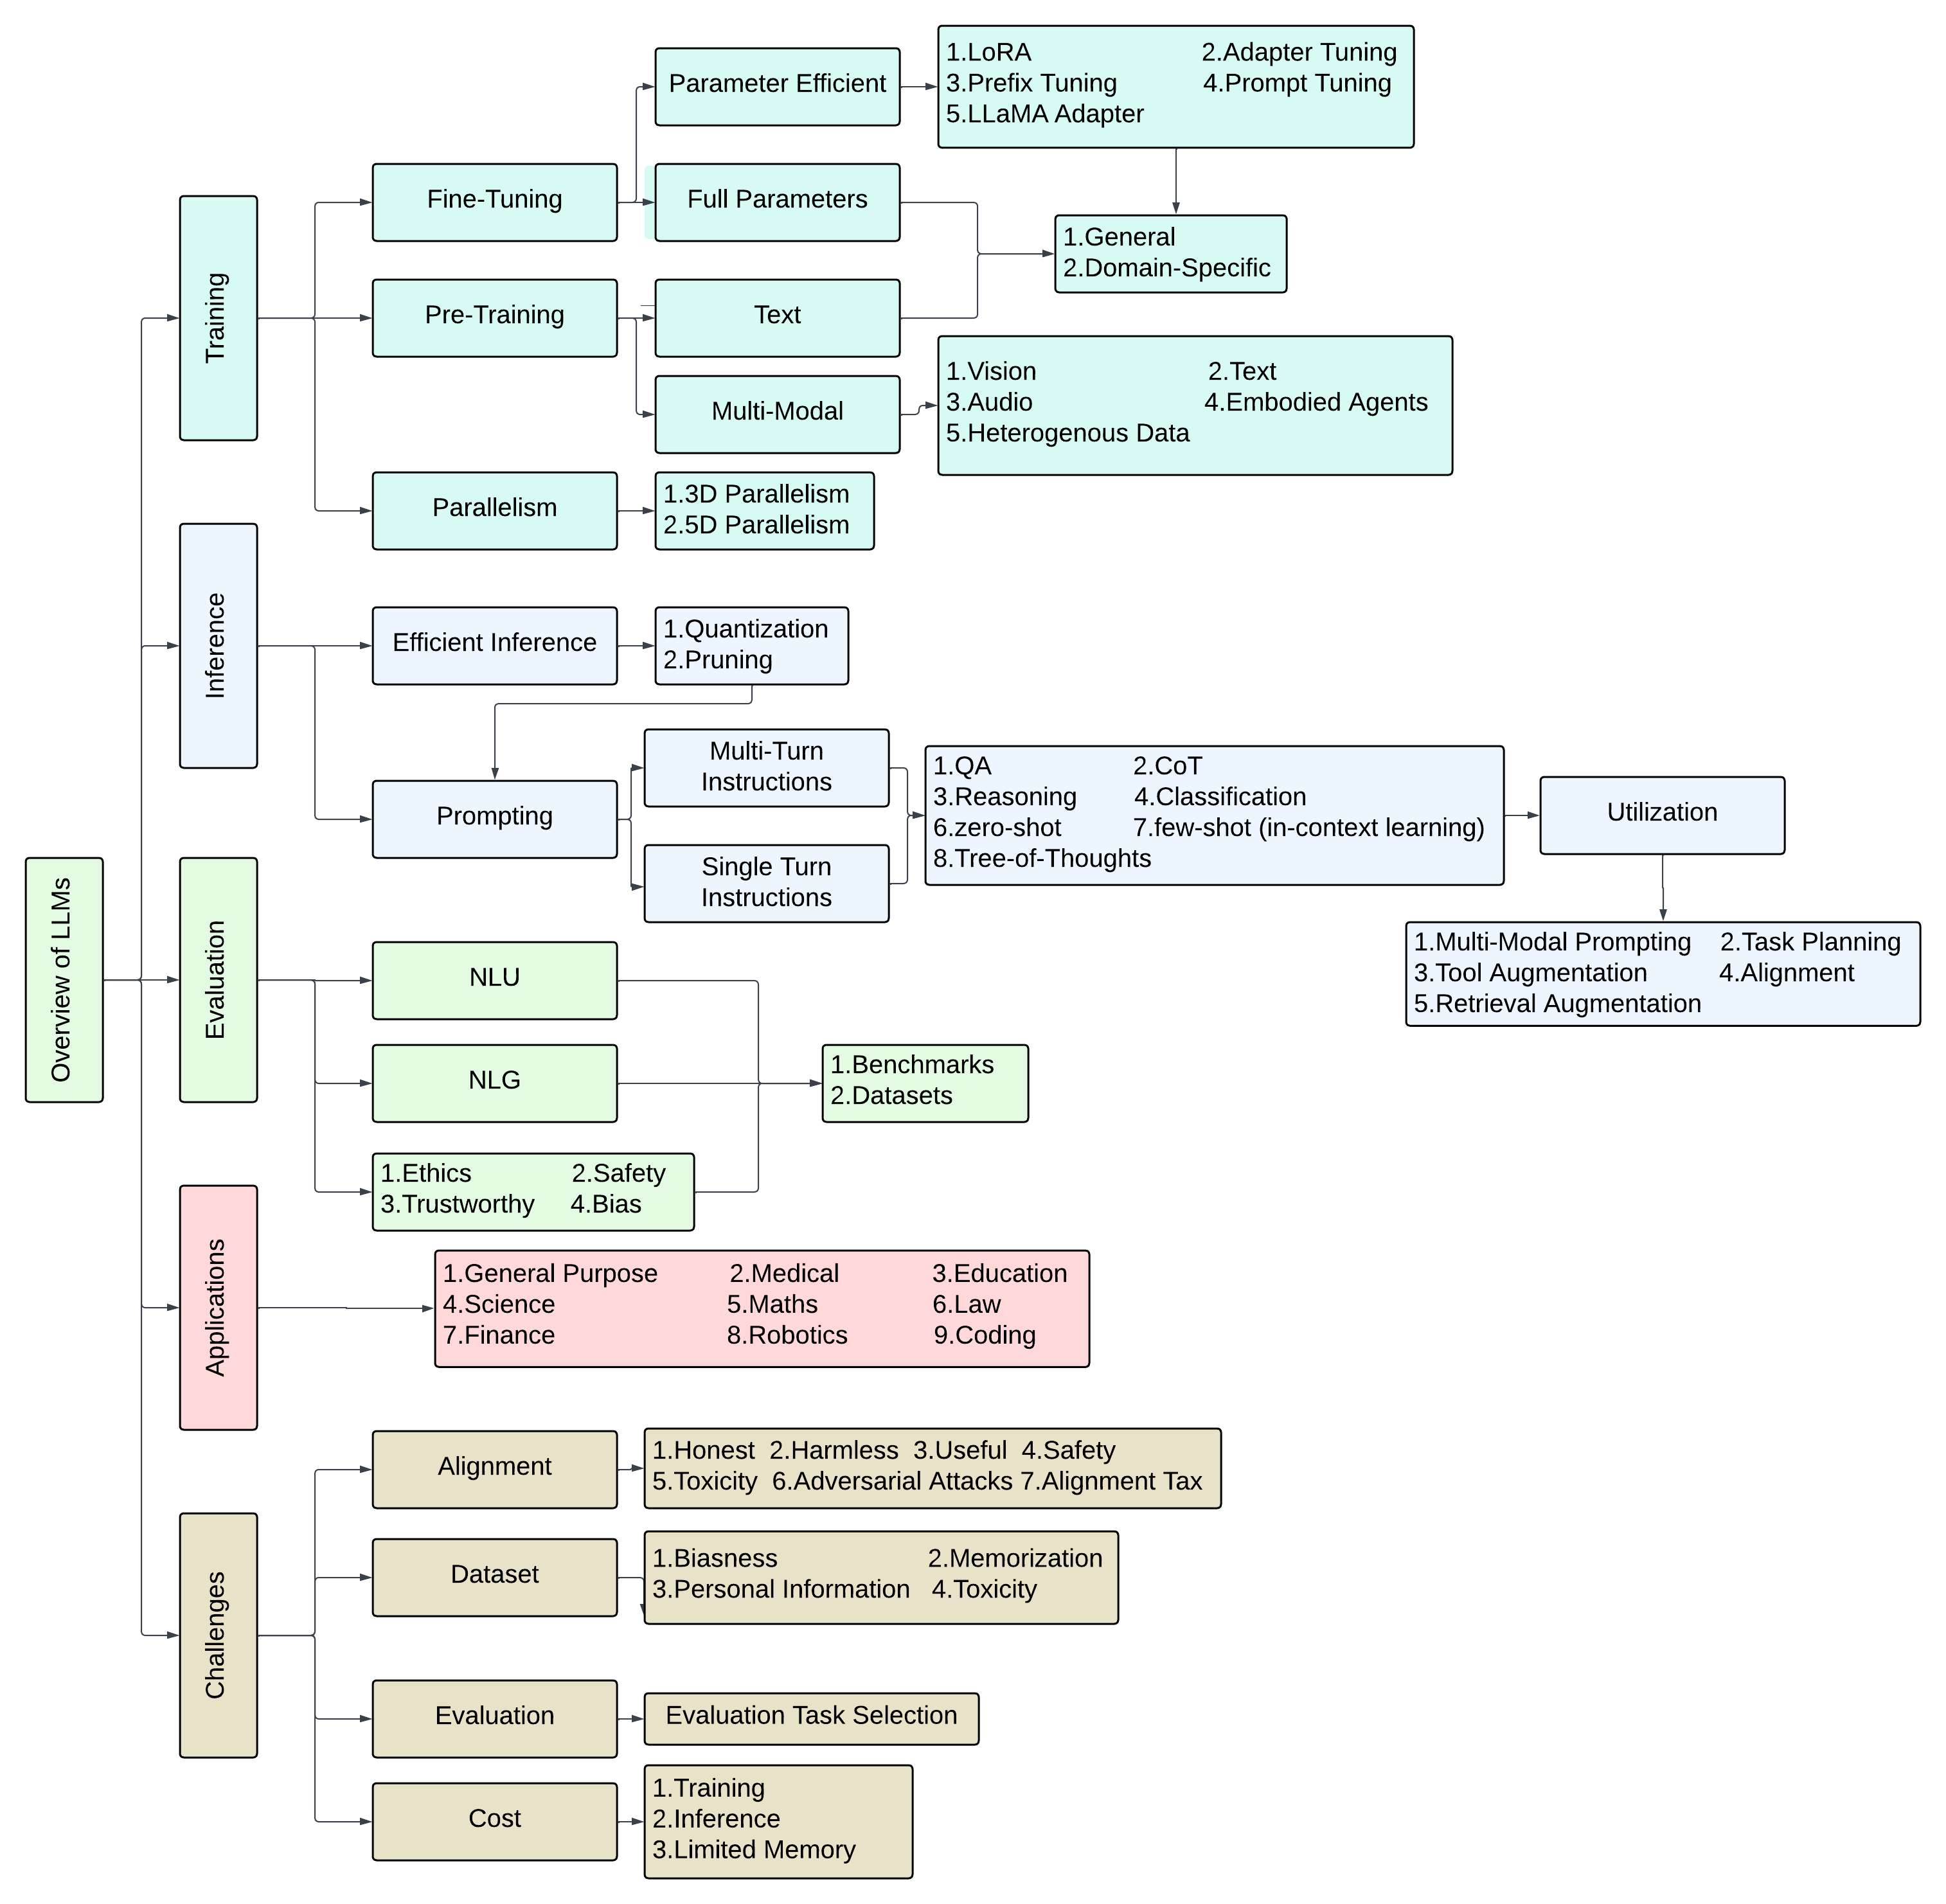
\includegraphics[width=\textwidth]{LLMs_Overview.png}
		}
		\centering
	\end{figure}
	\autocite{ACOoLLM}


\end{displayquote}

Large Language Models zijn heel complexe en extensieve implementaties, hierboven bij het citaat staat een diagram dat in vijf takken uitlegt hoe ze oppervlakkig in elkaar zitten.

\subsection{Keuze van een model}
Het kiezen van een model is iets dat van verschillende factoren afhangt:

\begin{itemize}
	\item \textbf{Modelgrootte en capabiliteit:} Grotere modellen geven meestal meer functionaliteiten en snellere werking maar dit ten koste van computerresources.
	\item \textbf{Datering van trainingsdata:} Oudere modellen die voorgetraind zijn op bepaalde data kunnen niet meer up-to-date zijn kunnen zo inaccurate antwoorden genereren.
	\item \textbf{Toegankelijkheid en kost:} Sommige modellen zijn betalend, terwijl sommige open-source modellen gratis te gebruiken zijn.
\end{itemize}

De keuze van een model hangt ook af van tijd; alles evolueert heel snel dus het is aangeraden om van tijd tot tijd te evalueren of ons model niet kan vervangen worden door iets nieuwer en capabeler.

Er zijn heel veel online providers van LLM apps zoals ChatGPT, Bard, Grok enz. 
Het probleem met cloudproviders is dat je met vertrouwelijke cliëntdata zit, deze wordt idealiter niet over het internet gestuurd naar een (gratis) LLM API. 

De keuze is dus, zoals eerder vermeld in deze paper, voor een lokaal model.
Deze zijn kneedbaar in implementatie en te verbinden met een vector store zoals degene die wij gebruiken. 


Nu neigt de keuze naar llama-3 van Meta: Een van de meest capabele modellen die openbaar verkrijgbaar zijn op dit moment.
\newpage
\section{Samenbrengen}
Nu de technologie van onze backend gekozen is, is het tijd om het samen te brengen in een entiteit die een input ontvangt en op basis van die input en de documentdatabase een output verschaft.

Een artikel van Jacob Lee op de blog van ollama.com wijst ons de weg op een straightforward manier.

\begin{displayquote}
	The general idea here is to take the user’s input question, search our prepared vectorstore for document chunks most semantically similar to the query,
	and use the retrieved chunks plus the original question to guide the LLM to a final answer based on our input data.

	There’s an additional step required for followup questions, which may contain pronouns or other references to prior chat history.
	Because vectorstores perform retrieval by semantic similarity, these references can throw off retrieval.
	Therefore, we add an additional dereferencing step that rephrases the initial step into a “standalone” question before using that question to search our vectorstore. 

	\begin{figure}[h]
		\makebox[\textwidth] {
			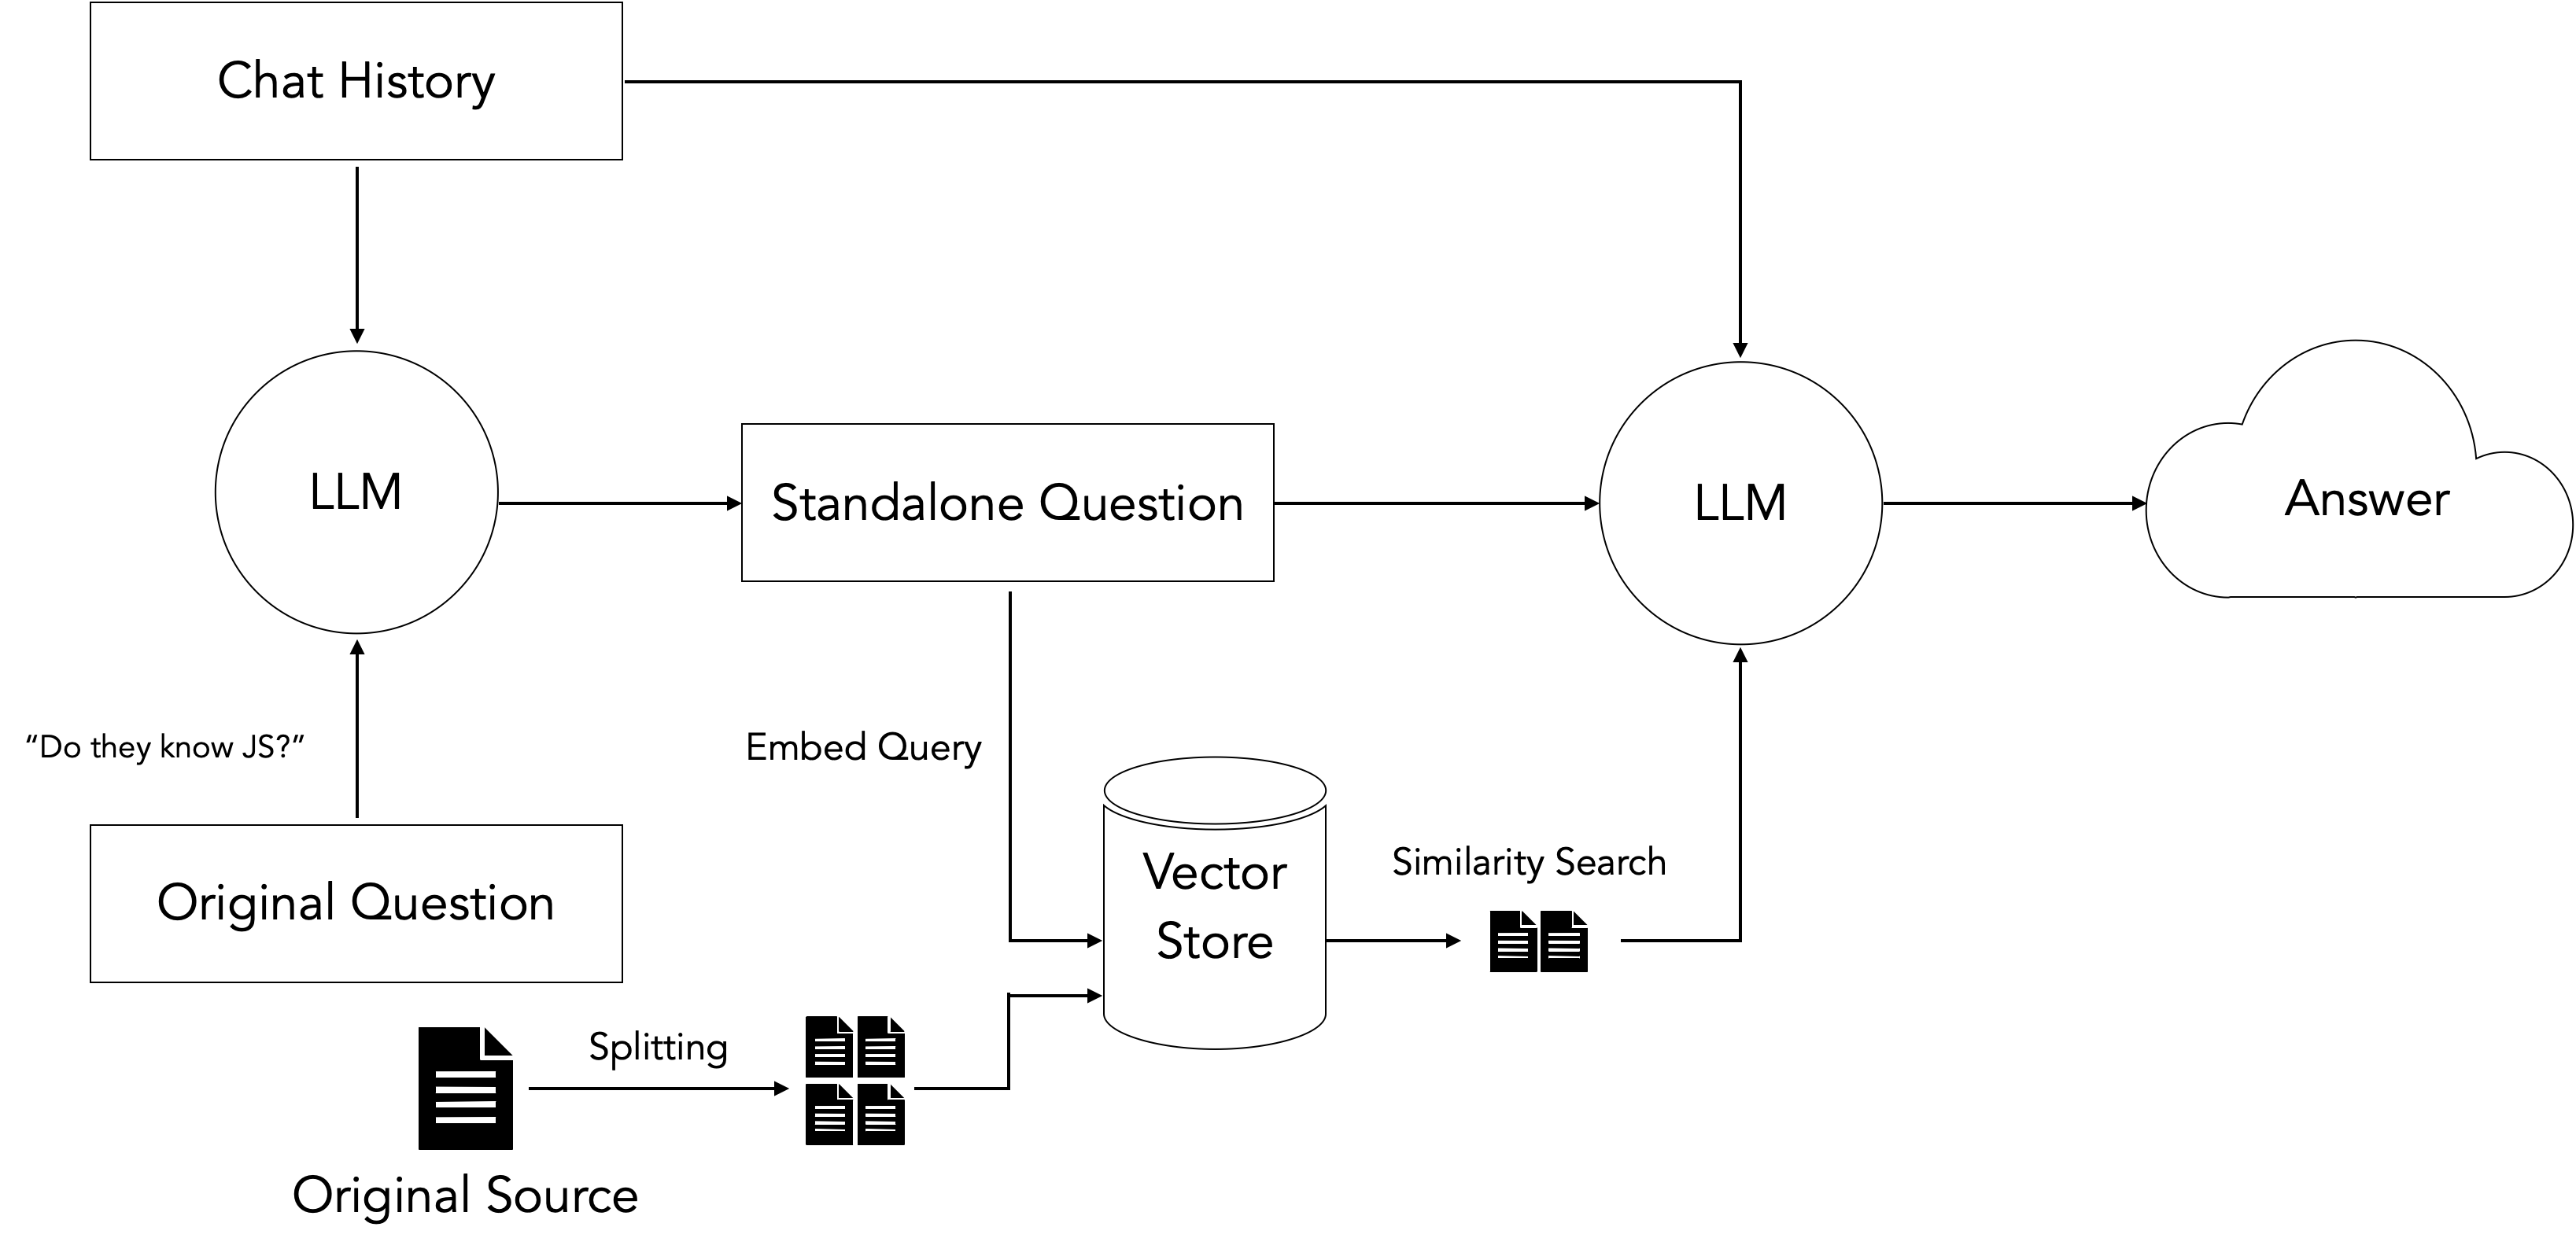
\includegraphics[width=\textwidth]{llm_pipeline.png}
		}
	\end{figure}
	\autocite{Ollama}
\end{displayquote}

Bovenstaande pipeline is een heel goeie richtlijn om onze implementatie op te baseren. Nu hebben we een interface nodig om queries in op te stellen als gebruiker en de outputs te kunnen lezen in een chat-achtige interface. 
